\section{AND Design} \label{sec:design}
In this section we describe the much improved design of {\sf AND}. Table \ref{tab:notation} introduces the relevant notation needed to understand the design in its entirety. 

\begin{table*}
\centering
\caption{Notation used in the presentation of this work.}
\label{tab:notation}
  \begin{tabular}{| r | l |} \hline
  $\mathsf{C}$ & Set of all consumers  \\
  $\mathsf{P}$ & Set of all producers  \\ 
  $\mathsf{R}$ & Set of all routers  \\
  $\mathsf{IF}$ & Set of all interfaces on all routers  \\
  $\mathsf{if}_i^r \in \mathsf{IF}$ & Interface $i$ of router $r$  \\
  $\kappa$ & The global security paramter (set to $256$ in practice) \\ 
  $(pk_i, sk_i)$ & Public/private key pair for router $r$  \\
  $\overline{\mathsf{int}}_{i}^{j}$ & Encrypted interest wrapped from router $i$ to router $j$ ($i \leq j$)  \\
  $\mathcal{A}$ & Adversary \\ 
  $u$ & Entity in the network (consumer or producer) \\
  $u \to_{\mathsf{int}} r$ & Entity $u$ sends interest to router $r$  \\ 
  $\mathsf{int} \to \mathsf{if}_i^r$ & Interest $\mathsf{int}$ is sent to interface $i$ of router $r$ \\
  $r \in \mathsf{R}$ & An anonymizing router (AR) \\ 
  $\mathcal{E}_{pk_i}(\cdot)$ & Public key encryption using $pk_i$ \\ 
  $\mathcal{D}_{pk_i}(\cdot)$ & Public key decryption using $pk_i$ \\ 
  $\mathsf{Encrypt}_{k_i}(\cdot)$ & Symmetric key encryption using key $k_i$ \\ 
  $\mathsf{Decrypt}_{k_i}(\cdot)$ & Symmetric key decrypt using key $k_i$ \\ 
  $\mathsf{ST}$ & AR session table used to store session ID and digest tuples \\
  $H$ & A collision resistant hash function on the domain $\{0,1\}^*$ to range $\{0,1\}^{\kappa}$ \\
  $F_k$ & A keyed pseudorandom function \\ \hline
  \end{tabular}
\end{table*}

\subsection{Circuit and Session Establishment}
At the heart of the {\sf AND} is the notion of anonymizing routers and connection-oriented circuits, similar in spirit to the inner workings of TOR \cite{Tor}. Anonymizing routers serve two purposes in {\sf AND}: (1) to decapsulate and forward encrypted interests, along with content encryption keys, generated by a consumer until the cleartext interest arrives at the producer, and (2) to encapsulate sensitive content using the previously acquired encryption keys and relay the encrypted content downstream. In this way, the consumer generates an interest wrapped by several layers of encryption and receives a piece of content wrapped in several layers of encryption that it can easily decrypt. It is also important to note that since each anonymizing router operates at the application layer, it effectively serves as the producer for each downstream router in the {\sf AND} circuit. Therefore, NDN policy dictates that such content \emph{must be signed}. Verification of content from upstream routers, however, is not mandatory. 

We also note that the current {\sf AND} design has support for two types of circuits: asymmetric and symmetric session-based. In the asymmetric variant, all encrypted interests are done using a CCA-secure PKI scheme and all content is encrypted using a CCA-secure symmetric key encryption scheme. Conversely, in the session-based variant, all encrypted interests are protected using a CCA-secure symmetric key encryption scheme, where the key is identified using a unique session identifier sent in the cleartext along with the encrypted interests. This worsens anonymity because it provides a way to link packets to a single session (as previously discussed).

Putting together all of the design aspects of the current version of {\sf AND}, we see that the following factors weigh in on the overall performance of the application: content encryption, content signature generation, and encrypted interest generation. In {\sf AND} we seek to minimize the degree to which these factors affect interest and content encapsulation and decapsulation by integrating support for anonymous router \emph{state}, which is encapsulated in sessions, into anonymous circuits. Sessions will exist for unidirectional traffic only, which therefore means that bidirection traffic, the ultimate focus of this work, will require two sessions to be established and maintained for the duration of the bidirectional application. This is done so that each party in the application need not use the same set of anonymous routers for communication. Not only does this free each consumer to select a random subset of anonymous routers $r_1,r_2,\dots,r_n$ from the set of total anonymous routers $\mathsf{R}$, but it may also help improve QoS guarantees by distributing the load of encapsulation and decapsulation among multiple nodes. Furthermore, sessions enable the establishment of long-term secrets that can be used to improve the efficiency of certain cryptographic operations, such as content encryption, signature generation, and signature verification. 

With the end of goal of supporting highly efficient and anonymous bidirectional traffic, the goals of the circuit and session establishment using a list of $n$ anonymous routers $r_1,\dots,r_n$ are as follows:
\begin{enumerate}
\item Establish unique session IDs $\mathsf{session}_{i}$ and session IVs $\mathsf{SIV}_i$
\item Establish content encryption keys $E_{k_i}$ and initial counter values $\mathsf{EIV}_i$
\item Establish pairwise MAC keys $M_{k_i}$ between adjacent routers and the consumer used to tag and verify content
\end{enumerate}

The purpose of each of these session entities will become clear from the circuit initialization and usage procedures. After establishment, the circuit from the consumer $C$ to the producer $P$ should be similar to that shown in Figure \ref{fig:circuit}. We now describe the general protocol for establishing this type of session-based circuit from a consumer $C$ to a producer $P$ given $n$ anonymous routers. Recall that, in order to support bidirectional communication, $P$ would have to establish a similar circuit to $C$ with $m$ routers, where $m$ need not equal $n$. 

{\sf AND} supports state initialization that is separate in time from circuit usage (i.e., using a handshake routine to initialize the state) as well as one that initializes session state upon issuance of the first wrapped consumer interest. In what follows we describe the handshake variant of session establishment. Online session establishment, used to remove the seemingly unnecessary handshake phase altogether, is discussed in Section \ref{sec:piggyback}.

\begin{algorithm*}[ht!]
  \caption{Circuit and Session Establishment Protocol}
  \begin{algorithmic}[1]
    \Require{Anonymous routers $r_1,r_2,\dots,r_n$ ($n \geq 1$) with public keys $pk_1,pk_2,\dots,pk_n$.}

% \Function{{\sf ServerRetrieveMACKey}}{$\mathsf{int}$} %// Server-side at router $i$
%   \State $(M_{k}, \mathsf{session}_i, x) := \mathcal{D}_{sk_i}(\mathsf{int}[-1])$ %// Recover MAC key and randomness $x$
%   \If{$\mathsf{session}_i$ not in state}
%     \State \Return $\mathsf{Error}$
%   \Else
%     \State Persist $M_k$ as $M_{k_{i+1}}$ (the upstream MAC key) with session $\mathsf{session}_i$
%     \State $x^* := \mathsf{MAC}_{M_{k}}(x)$
%     \State $\mathsf{resp} := x^*$
%     \State \Return $\mathsf{resp}$
%   \EndIf

%   % \State $(E_{k_n}, M_{k_n}, \mathsf{EIV}_n, \mathsf{session}_n, \mathsf{SIV}_n) \gets \overline{\mathcal{D}_{k}}(T)$
%   % \State \Return $(E_{k_n}, M_{k_n}, c_n, \mathsf{session}_n, \mathsf{IV}_n)$
% \EndFunction

\medskip

\Function{{\sf ServerEstablishSession}}{$\mathsf{int}$} %// Server-side at router $i$
  % \State $k \gets \mathcal{D}_{sk_i}(\mathsf{int}[-1])$ %// Recover session encryption key
  % \State $E_{k_i} \gets \{0,1\}^{\kappa}$ %// Encryption key
  % \State $M_{k_i} \gets \{0,1\}^{\kappa}$ %// MAC key
  % \State $\mathsf{EIV}_i \gets \{0,1\}^{\kappa}$ %    // counter IV
  % \State $x \gets \{0,1\}^{\kappa}$
  % \State $\mathsf{SIV}_i \gets \{0,1\}^{\kappa}$ %// session IV
  % \State $\mathsf{session}_i := H(x)$ %// session ID
  % \State $\mathsf{SIndex}_i := H(\mathsf{session}_i + \mathsf{SIV}_i)$
  \State $(k, E_{k_i}, M_{k_i}, M_{k_{i+1}}, \mathsf{EIV}_i, \mathsf{SIV}_i, \mathsf{session}_i, \mathsf{SIndex}_i) := \mathcal{D}_{sk_i}(\mathsf{int})$
  \State Persist $(\mathsf{session}_i, E_{k_i}, M_{k_i}, M_{k_{i+1}}, \mathsf{EIV}_i, \mathsf{SIV}_i)$ to state, and store $(\mathsf{SIndex}_i, \mathsf{session}_i, \mathsf{SIV}_i)$ in the session table $\mathsf{ST}_i$
  \State $\mathsf{resp} \gets \mathsf{Encrypt}_{k}(\mathsf{session}_i, E_{k_i}, M_{k_i}, \mathsf{EIV}_i, \mathsf{SIV}_i)$
  \State \Return $\mathsf{resp}$
  
  % \State $T' := \mathcal{D}_{sk}(T)$ // Secret key $sk$ corresponding to the receiving router $r$
  % \If {$|T'| = 4$}
  %   \State Persist $(\mathsf{session}, E_{k}, c, M_{k})$ to state
  % \Else
  %   \State Persist $(\mathsf{session}, E_{k}, c, M_{k}, M_{k_{+1}})$ to state
  % \EndIf
\EndFunction

\medskip

% \Function{{\sf ClientSendMACKey}}{$r_i$, $\mathsf{session}_i$, $M_{k}$} // Client-side
%   \State $x \gets \{0,1\}^{\kappa}$
%   \State $x' := \mathsf{MAC}_{M_{k}}(x)$
%   \State $T \gets \mathcal{E}_{pk_i}(M_{k}, \mathsf{session}_i, x)$
%   \State $\mathsf{int} := \mathsf{namespace}_i/\mathsf{SESSIONMAC}/T$
%   \State $\mathsf{resp} := \mathsf{ccnget}(\mathsf{int})$ // reach out to the AR
%   \State $x^* := \mathsf{resp}[-1]$
%   \If{$x' \not= x^*$}
%     \State \Return $\mathsf{Fail}$
%   \Else
%     \State \Return $\mathsf{Pass}$
%   \EndIf

%   % \State $(E_{k_n}, M_{k_n}, \mathsf{EIV}_n, \mathsf{session}_n, \mathsf{SIV}_n) \gets \overline{\mathcal{D}_{k}}(T)$
%   % \State \Return $(E_{k_n}, M_{k_n}, c_n, \mathsf{session}_n, \mathsf{IV}_n)$
% \EndFunction

\Function{{\sf ClientEstablishSession}}{$r_i$, $M_{k_{i+1}}$} %// Client-side
  % \State $k \gets \{0,1\}^{\kappa}$
  % \State $\overline{k} \gets \mathcal{E}_{pk_i}(k)$

  % \State $k \gets \mathcal{D}_{sk_i}(\mathsf{int}[-1])$ %// Recover session encryption key
  \State $E_{k_i} \gets \{0,1\}^{\kappa}$ %// Encryption key
  \State $M_{k_i} \gets \{0,1\}^{\kappa}$ %// MAC key
  \State $\mathsf{EIV}_i \gets \{0,1\}^{\kappa}$ %    // counter IV
  \State $x \gets \{0,1\}^{\kappa}$
  \State $\mathsf{SIV}_i \gets \{0,1\}^{\kappa}$ %// session IV
  \State $\mathsf{session}_i := H(x)$ %// session ID
  \State $\mathsf{SIndex}_i := H(\mathsf{session}_i + \mathsf{SIV}_i)$

  \State $\mathsf{int} := \mathsf{namespace}_i/\mathsf{CREATESESSION}/\mathcal{E}_{pk_i}(k, E_{k_i}, M_{k_i}, M_{k_{i+1}}, \mathsf{EIV}_i, \mathsf{SIV}_i, \mathsf{session}_i, \mathsf{SIndex}_i)$
  \State $\mathsf{resp} := \mathsf{ccnget}(\mathsf{int})$ // reach out to the AR
  % \State $(E_{k_n}, M_{k_n}, \mathsf{EIV}_n, \mathsf{session}_n, \mathsf{SIV}_n) \gets \mathsf{Decrypt}_{k}(\mathsf{resp})$
  \State \Return $(E_{k_i}, M_{k_i}, x_i, \mathsf{session}_i, \mathsf{IV}_i)$
\EndFunction

% \State $E_{k_i} \gets \{0,1\}^k$ for $k = 1,\dots,n$ // Encryption key
% \State $M_{k_i} \gets \{0,1\}^k$ for $k = 1,\dots,n$ // MAC key
% \State $c_i \gets \{0,1\}^k$ for $k = 1,\dots,n$     // counter IV
% \State $x \gets \{0,1\}^k$
% \State $\mathsf{session}_n := H(x)$
% \State $T' := (\mathsf{session}_n, E_{k_n}, c_n, M_{k_n})$
% \State $T_n := \mathcal{E}_{pk_n}(T')$

\medskip

\Function{{\sf EstablishCircuit}}{$r_1,\dots,r_n$} %// Main procedure
\State $(E_{k_n}, M_{k_n}, c_n, \mathsf{session}_n, \mathsf{IV}_n) := \mathsf{ClientEstablishSession}(r_n)$
\For{$i = n - 1$ \textbf{ downto } $1$}
  \If{$i = n-1$}
    \State $(E_{k_i}, M_{k_i}, \mathsf{EIV}_i, \mathsf{session}_i, \mathsf{SIV}_i) := \mathsf{ClientEstablishSession}(r_i, \perp)$
  \Else
    \State $(E_{k_i}, M_{k_i}, \mathsf{EIV}_i, \mathsf{session}_i, \mathsf{SIV}_i) := \mathsf{ClientEstablishSession}(r_i, M_{k_{i+1}})$
  \EndIf
  % \If{$\mathsf{ClientSendMACKey}(r_i, \mathsf{session}_i, M_{k_{i+1}}) = \mathsf{Fail}$}
    % \State \Return $\mathsf{Fail}$
  % \EndIf
  % \State $\mathsf{session}_{i} := H(\mathsf{session}_n \bigoplus_{j=i}^{n} E_{k_j})$
  % \State $T' := (\mathsf{session}_i, E_{k_i}, c_i, M_{k_i}, M_{k_{i+1}})$
  % \State $T_n := \mathcal{E}_{pk_i}(T_i)$
  % \State $\mathsf{EstablishSession}(T_i)$
\EndFor
\EndFunction

  \end{algorithmic}
\end{algorithm*}

Notice that by this procedure, no two routers will share the same session identifier (with non-negligible probability) even though they partake in the same circuit. This is because they generate session identifiers independent and uniformly at random from $\{0,1\}^{\kappa}$. 

% \begin{figure*}[ht!]
% \begin{center}
% 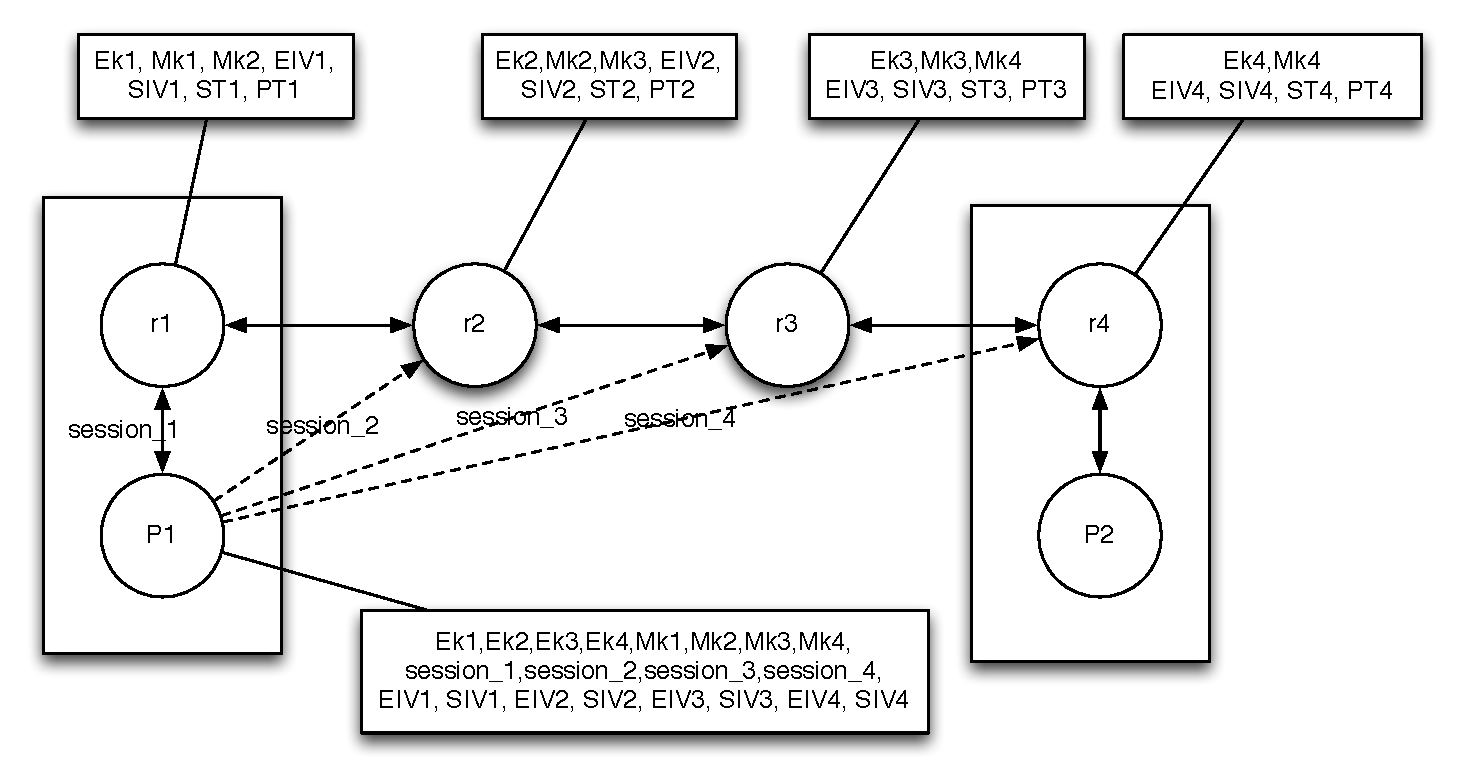
\includegraphics[scale=0.5]{./images/circuit.pdf}
% \end{center}
% \caption{Sample session-based circuit between a consumer $C$ and producer $P$ with ARs $r_1,r_2,r_3,r_4$, where the end routers on the path are run on the same node as $C$ and $P$.}
% \label{fig:circuit}
% \end{figure*}

\subsection{AND Circuit Usage}

We note that anonymous routers must be chosen in a \emph{mutually excluse} manner, meaning that they do not change share the same name prefix or are from the same organization (see Figure \ref{fig:pool}). This requirement is needed for ensuring anonymity. After a circuit and the corresponding sessions have been created between the consumer and each anonymous router, usage of the circuit proceeds as per the original {\sf AND} design. Specifically, there are three main operations that need to be defined: encrypted interest generation, AR interest forwarding, and AR content handling. In what we follows we present the details of each of these procedures as needed for {\sf AND}. We begin with the encrypted interest generation procedure (shown in Algorithm \ref{alg:enc_int_gen}) in which a consumer $C$ particpating in a particular \emph{application} session with a producer $P$ wraps an interest for the session to be sent into the anonymizing circuit. A wrapped (encrypted) interest from $r_i$ to $r_j$ ($i \leq j$) is denoted as $\overline{\mathsf{int}}_i^j$, meaning that the original plaintext interests $\mathsf{int}$ cannot be retrieve unless encrypted by each router $r_i,r_{i+1},\dots,r_j$, in that order. Thus, the original wrapped interest is denoted as $\overline{\mathsf{int}}_1^n$.

\begin{figure*}[ht!]
\begin{center}
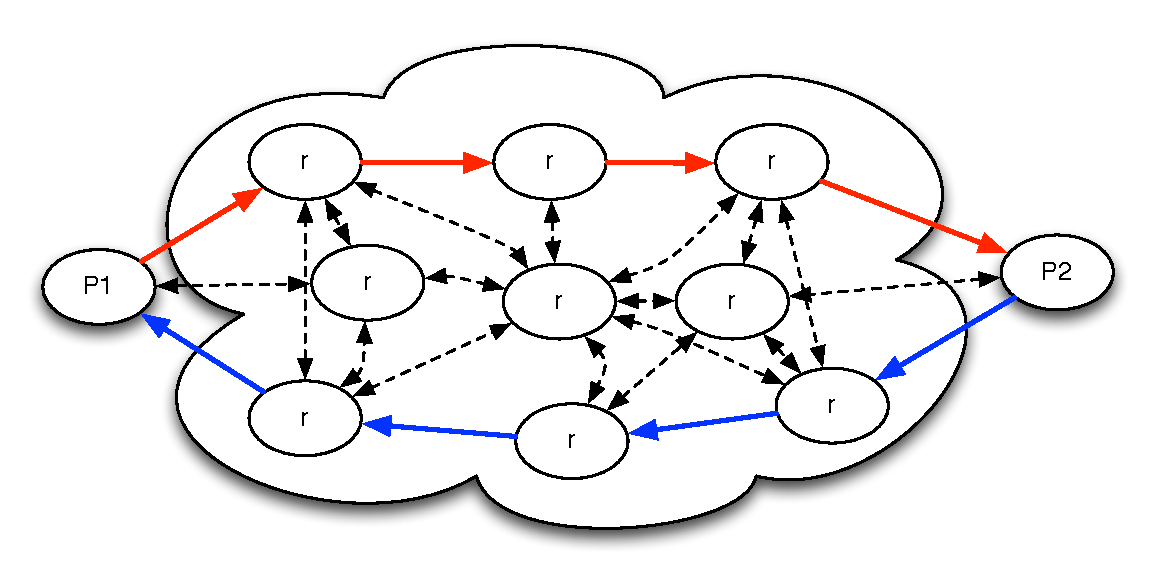
\includegraphics[scale=0.5]{./images/pool.pdf}
\end{center}
\caption{A sample bidirectional circuit configuration in which two parties communicate using mutually exclusive ARs in both directions. Note that it is not required for each circuit to be the same length, nor is it required that the intersection of the routers for each direction of the circuit to be empty (i.e., routers may \emph{unknowingly} support sessions traversing in both directions).}
\label{fig:pool}
\end{figure*}

\begin{algorithm}[ht!]
  \caption{Encrypted Interest Generation}
  \begin{algorithmic}[1]
    \Require{Interest $\mathsf{int}$, circuit length $n$, AR pool $\mathcal{R}$}
    \Ensure{Encrypted interest $\overline{\mathsf{int}}_{1}^{n}$}
\State $\overline{\mathsf{int}} = \mathsf{int}$
\For{$i = n$ \textbf{ downto } $1$}
  \State $\mathsf{SIndex}_i := H(\mathsf{session}_i + \mathsf{SIV}_i)$
  \State $\mathsf{SIV}_i = \mathsf{SIV}_i + 1$ (mod $2^{\kappa}$)
  \State $\overline{\mathsf{int}}_i^n = R_i / \mathsf{SIndex}_i / \mathsf{Encrypt}_{E_{k_i}}(\overline{\mathsf{int}}, \mathsf{timestamp})$
\EndFor
\State \Return $\overline{\mathsf{int}}_1^n$
\end{algorithmic}
\label{alg:enc_int_gen}
\end{algorithm}

\begin{algorithm*}[ht!]
  \caption{AR Encrypted Interest Forwarding}
  \begin{algorithmic}[1]
    \Require{$\overline{\mathsf{int}}_i^j$}
    \Ensure{$(\overline{\mathsf{int}}_{i+1}^j, \mathsf{session}_i)$ or discarded packet}
\If{$\mathsf{SIndex}_i \in \mathsf{ST}_i$}
  \State Let $(\mathsf{session}_i, E_{k_i}, M_{k_i}, \mathsf{EIV}_i, \mathsf{SIV}_i)$ be the session information associated with $\mathsf{SIndex}_i$
  \State $\mathsf{SIV}_i := \mathsf{SIV}_i + 1$ (mod $2^{\kappa}$)
  \State $\mathsf{SIndex}_i := H(\mathsf{session}_i + \mathsf{SIV}_i)$
  \State Update $(\mathsf{SIndex}_i, \mathsf{session}_i, \mathsf{SIV}_i)$ in the session table $\mathsf{ST}_i$
  \State $(\overline{\mathsf{int}}_{i+1}^{j}, timestamp) := \mathsf{Decrypt}_{E_{k_i}}(\overline{\mathsf{int}}_{i}^{j})$
  \If{decryption fails or $\mathsf{timestamp}$ is not current}
    \State Discard $\overline{\mathsf{int}}_{i}^{j}$
  \Else
    \State Persist tuple $T_i = (\overline{\mathsf{int}}_{i}^{j}, \overline{\mathsf{int}}_{i+1}^{j}, \mathsf{session}_i)$ to pending interest table $\mathsf{PT}_i$
    \State \Return $(\overline{\mathsf{int}}_{i+1}^{j}, \mathsf{session}_i)$
  \EndIf
\Else
  \State Discard $\overline{\mathsf{int}}_{i}^{j}$ %\Comment{Some form of interest flooding prevention should be employed here}
\EndIf
\end{algorithmic}
\label{alg:enc_int_forward}
\end{algorithm*}

\begin{algorithm}[ht!]
  \caption{AR Content Handling}
  \begin{algorithmic}[1]
    \Require{Content $\overline{data_{i+1}^j}$ in response to interest $\overline{\mathsf{int}}_{i+1}^{j}$}
    \Ensure{Encrypted data packet $data_{i}^j$}
\State Recover tuple $T_i = (\overline{\mathsf{int}}_{i}^{j}, \overline{\mathsf{int}}_{i+1}^{j}, \mathsf{session}_i)$ based on $data_{i+1}^j$
\State Parse $\overline{data_{i+1}^j}$ as a tuple $(data_{i+1}^j, \sigma_{i+1})$
\If{$\sigma_{i+1} = \epsilon$ and $M_{k_{i+1}} = \epsilon$} %\Comment{Last hop router - does not verify MAC}
  \State Pass
\ElsIf{$\sigma_{i+1} \not= \epsilon$ and $M_{k_{i+1}} \not= \epsilon$}
  \If{$\sigma_{i+1} = \mathsf{Verify}_{M_{k_{i+1}}}(data_{i+1}^j)$}
    \State Pass
  \Else
    \State \Return $\mathsf{Error}$ %\Comment{MAC verification did not pass}
  \EndIf
\Else %\Comment{There was either a tag or we don't have the upstream MAC key - either way, we error}
  \State \Return $\mathsf{Error}$
\EndIf

\State Remove signature and name from $data_{i+1}^j$    
\State Create new empty data packet $data_i^j$
\State Set name on $data_i^j$ as the name on $\overline{\mathsf{int}}_{i}^{j}$
\State $data_i^j := \mathsf{Encrypt}_{E_{k_i}}(data_i^j)$
\State $\sigma_i := \mathsf{MAC}(data_i^j)$
\State $\overline{data_{i}^j} = (data_i^j, \sigma_i)$
\State \Return $\overline{data_{i}^j}$

\end{algorithmic}
\label{alg:ar_content_handler}
\end{algorithm}

% \begin{figure*}[ht!]
% \begin{center}
% 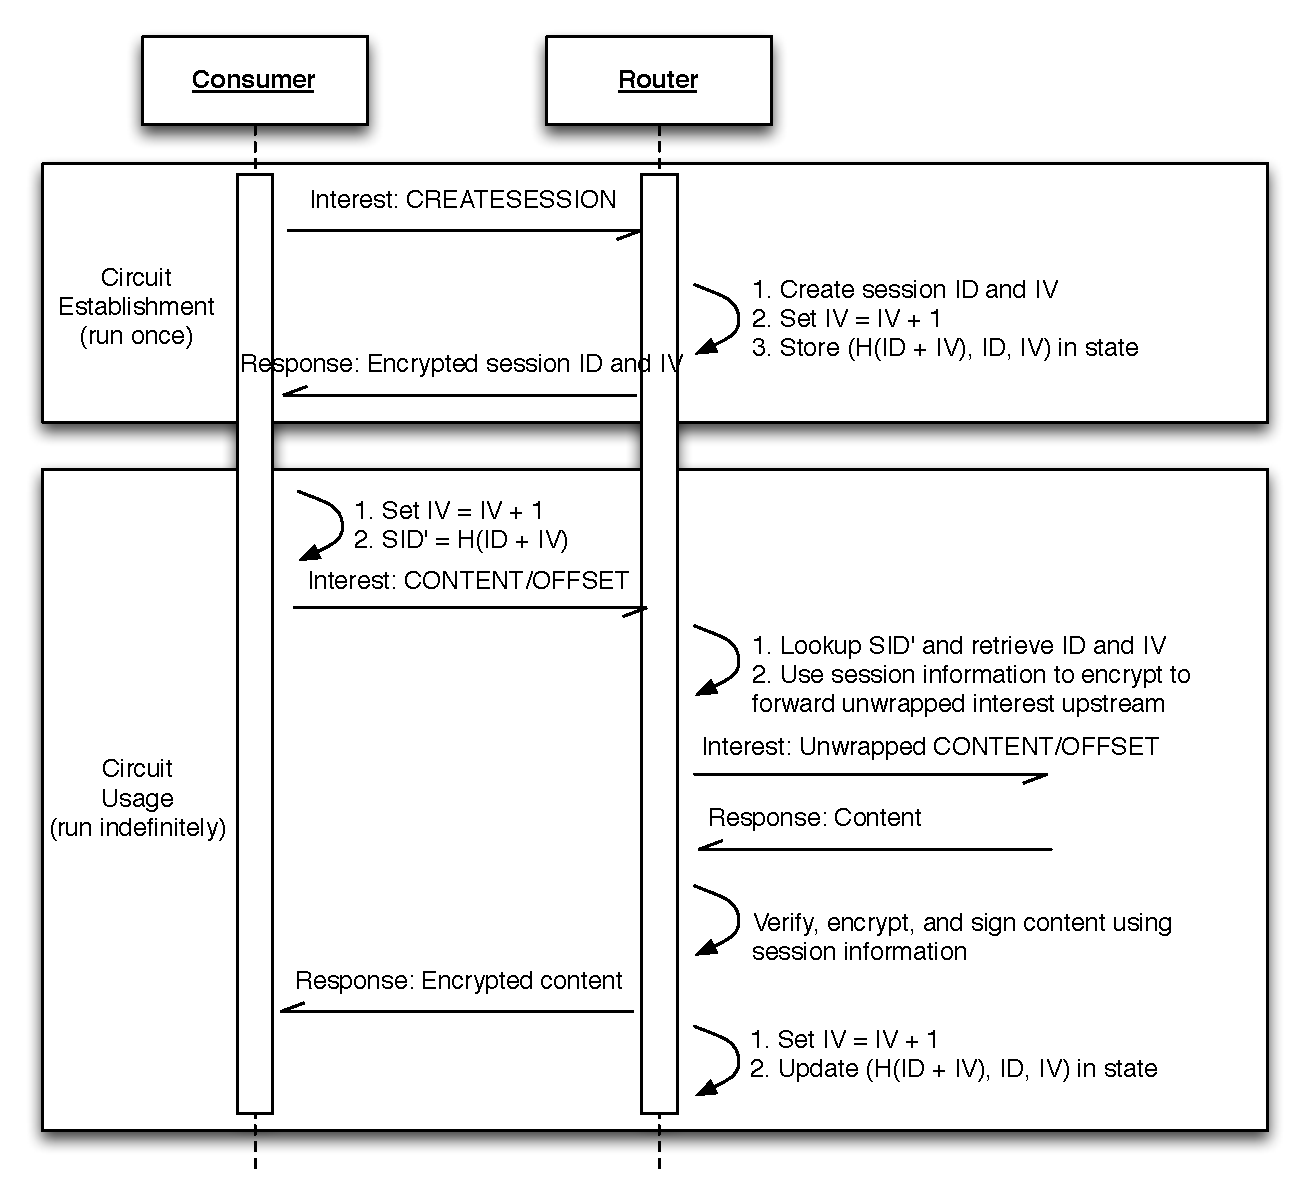
\includegraphics[scale=0.65]{./images/circuit_usage.pdf}
% \end{center}
% \caption{Visual depiction of the interaction between the consumer and the first hop router for the handshake-based variant. The procedure repeats in the same manner for all further upstream routers after each interest is unrolled and resulting content is encrypted.}
% \label{fig:circuit_usage}
% \end{figure*}

\subsection{Online Session Establishment and Circuit Usage} \label{sec:piggyback}
As previously mentioned, sessions may be created via the handshake technique or online. The process for online state initialization is very similar to the handshake routine with the following exceptions:
\begin{itemize}
  \item The \emph{first} interest $\mathsf{int}$:$1$ issued by the consumer is appended with the encrypted state information (minus the session index) similar to as is done in the handshake variant. The session index $\mathsf{SID}$ is still appended to the interest before the state information. This enables the anonymizing proxies to check for the presence of the session index in their state table. If an entry is not found, the remainder of the interest is decrypted and treated as the initial state information.
  \item All \emph{subsequent} interests $\mathsf{int}$:$i$ ($i > 1$) are prepended with the session index and \emph{padded} with an $l$ bits of data so that $|\mathsf{int}$:$1| = |\mathsf{int}$:$i|$ (i.e., the length of all interests are equal). Since the concatenation of the session identifier and the state information is indistinguishable from the concatenation of a different session identifer and random pad, an adversary cannot distinguish between $\mathsf{int}$:$1$ and $\mathsf{int}$:$i$.
\end{itemize}
Beyond these changes, the operation and usage of the circuits remains the same for consumers and anonymizing proxies. We omit algorithmic details about the above differences since they should be clear from context.

\subsection{Interest Flow Control via Windowing} \label{sec:windowing}
To further increase the throughput of {\sf AND}, the design makes use of a flow control mechanism analogous to the sliding window technique used in standard TCP implementations. In particular, {\sf AND} uses a global maximum window size $w$ that refers to the maximum number of interests that can be issued asynchronously without being acknowledged. The behavior of the interest sliding window will then proceed as follows:
\begin{itemize}
  \item All parties, including the consumer and each AR participating in an anonymous circuit, will maintain four pointers, $\mathsf{WindowStart}$, $\mathsf{WindowEnd}$, $\mathsf{KeyStart}$, and $\mathsf{KeyEnd}$, where $\mathsf{WindowEnd} - \mathsf{WindowStart} \leq w$ will always be an invariant. To start, $\mathsf{WindowStart} = \mathsf{WindowEnd} = 0 = \mathsf{KeyStart} = \mathsf{KeyEnd} = 0$.
  \item When an interest is to be issued or forwarded, the party will check to ensure that $\mathsf{WindowEnd} - \mathsf{WindowStart} < w$, and if so interest is sent/forwarded and $\mathsf{WindowEnd}$ is incremented by one. In addition, the keystream at the consumer (for each AR) or AR is pumped by $M$ bits and $\mathsf{KeyEnd}$ is incremented by $M$, where $M$ is the largest piece of content received thus far. Otherwise, the interest is buffered at the consumer or AR. 
  \item When a piece of content arrives that corresponds to some interest issued between $\mathsf{WindowStart}$ and $\mathsf{WindowEnd}$, $\mathsf{WindowStart}$ is incremented by one and an event is triggered forcing the party to check their interest buffers for new intersts to be sent. In addition, $\mathsf{KeyStart}$ is incremented by the size of the content, and checks to see if the maximum content size $M$ needs to be updated.
\end{itemize}
Using this technique, if a router receives an interest for a particular anonymous circuit when $\mathsf{WindowEnd} - \mathsf{WindowStart} \geq w$, then the interest is dropped. Interest and content flow control and correct functionality of the consumer guarantees that interests will not be issued when the window is full. 

Also, while all parties must share the same window size, the consumer $w$ is free to change the window size to adapt to the state of the network. For instance, if there is very little end-to-end latency for content, then the consumer may wish to increase the size of the window. In order to support such dynamic windowing, the consumer must inform all routers in an anonymous circuit of the desired window size. {\sf AND} supports this by appending the window size to the session index $\mathsf{SIndex}_i$ for each $r_i$ in a circuit. In order to ensure that no two interests are distinguishable by this window size $w$, it is also masked by a random one-time pad $p$ (i.e. $w' = w \oplus p$, where $w$ is interpreted as an integer encoded in binary) that is included in the encrypted interest. In other words, once an interest is decrypted the pad $p$ is recovered, and then the router computes $w = w' \oplus p$. If $w$ is larger than the stored value associated with the circuit, then the new result is simply updated and operation proceeds as normal. Otherwise, the router enters a ``backoff'' state where it waits for content to be returned and the resulting window size to return to normal before issuing any further interests. This dynamic windowing method is currently not implemented in the {\sf AND} system.

\begin{figure*}[ht!]
\begin{center}
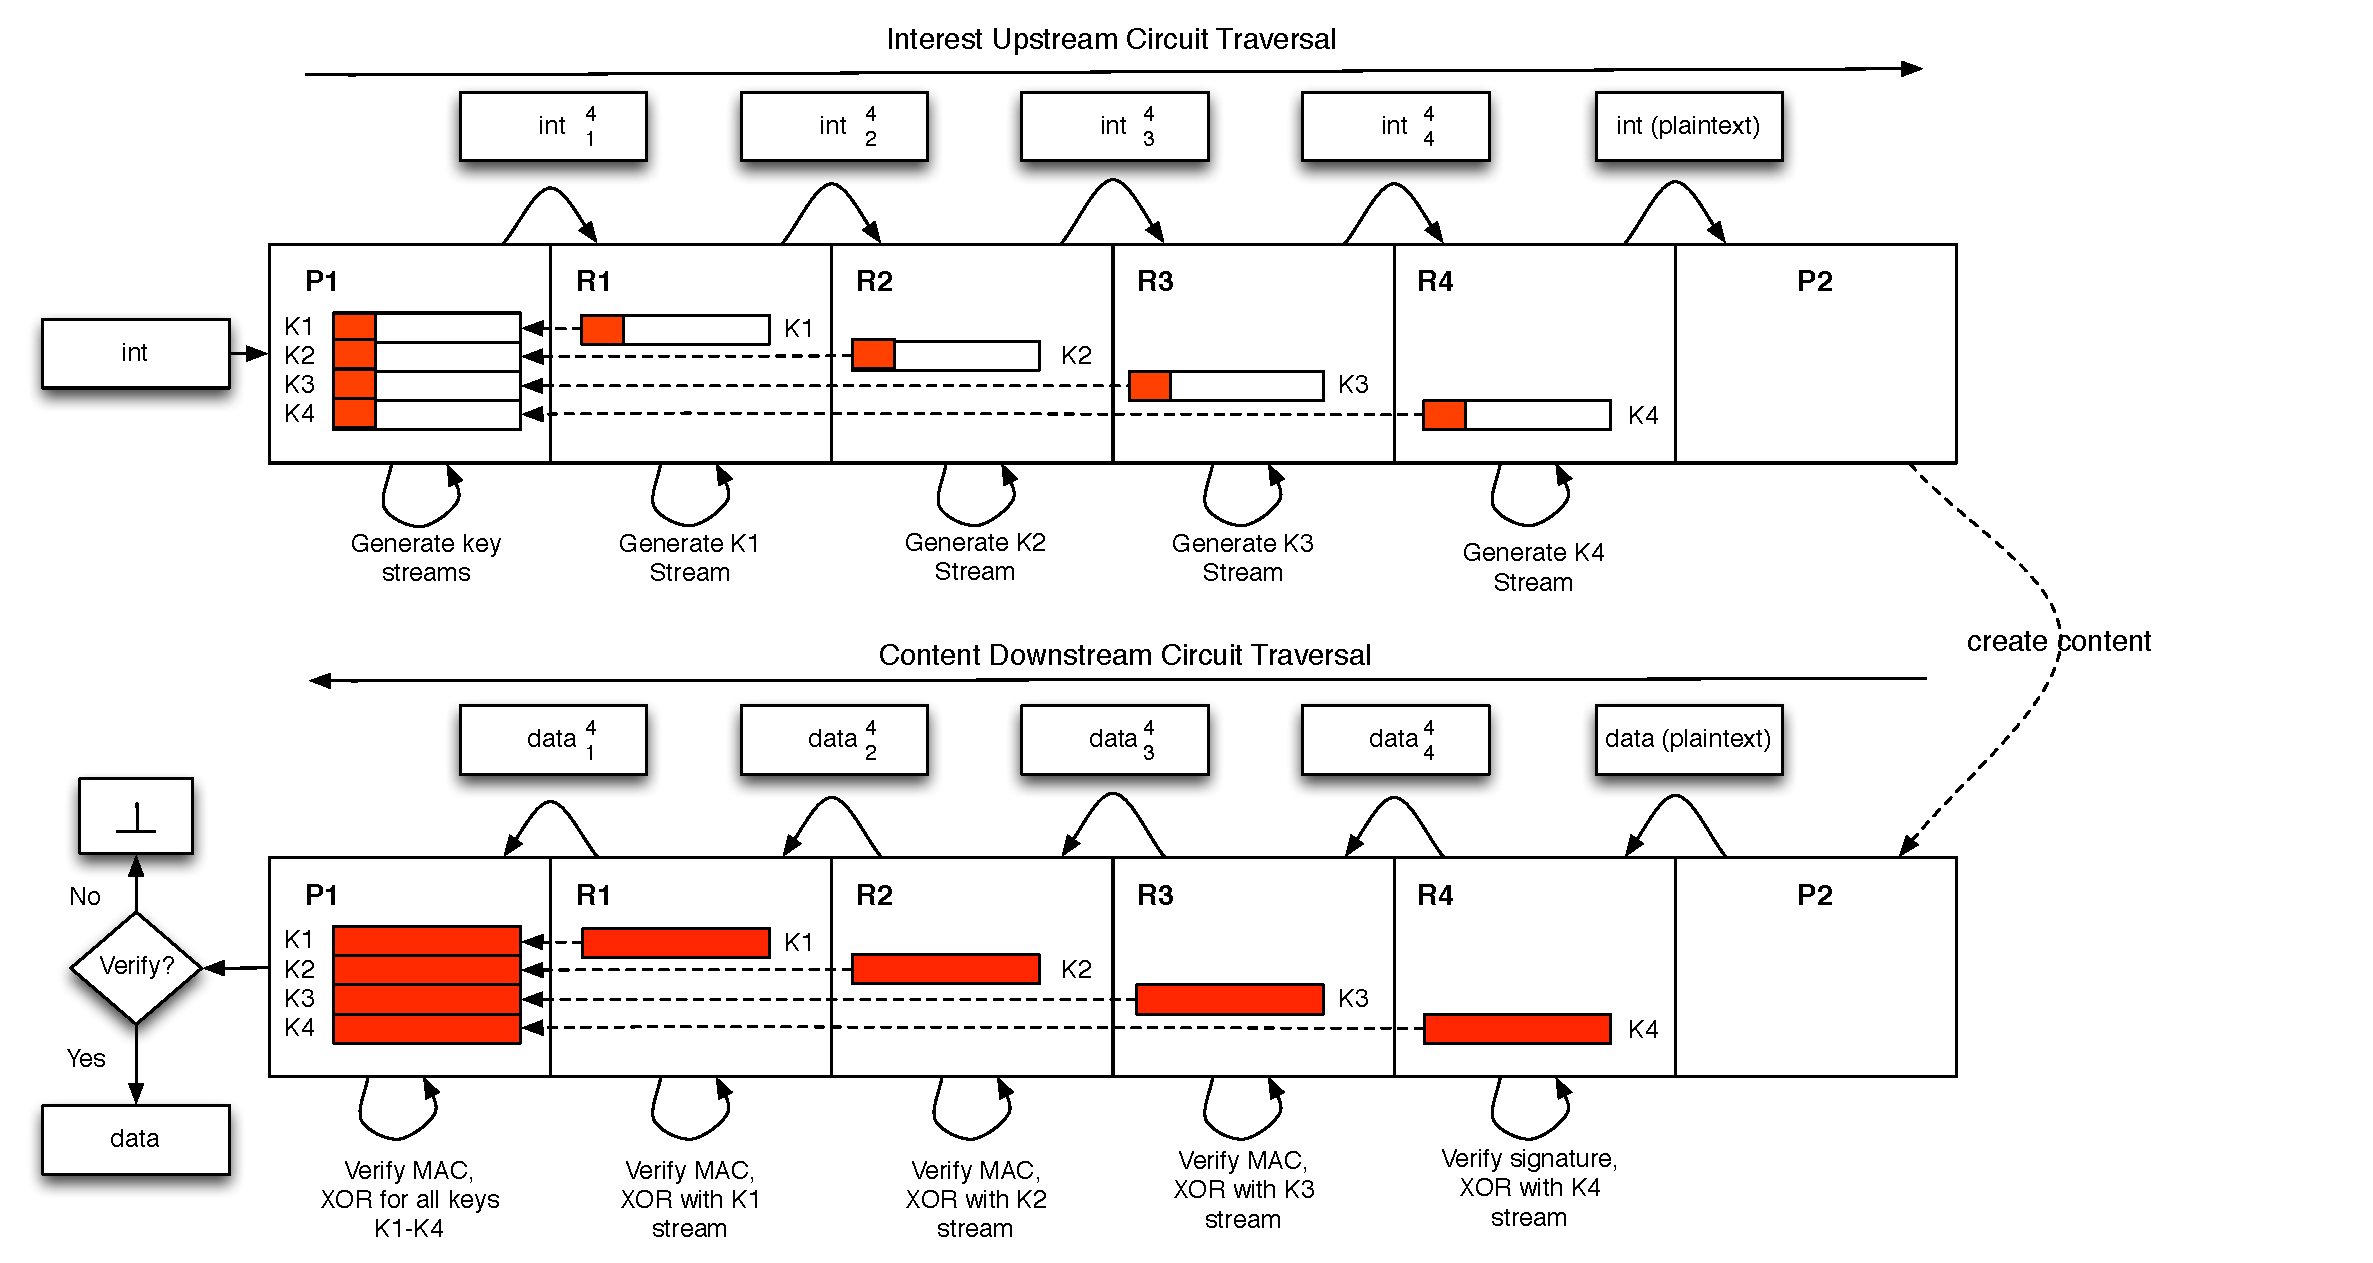
\includegraphics[scale=0.45]{./images/ctr_split.pdf}
\end{center}
\caption{Visual depiction of window-based keystream precomputation during upstream interest traversal.}
\label{fig:circuit}
\end{figure*}
